%%%%%%%%%%%%%%%%%%%%%%%%%%%%%%%%%%%%%%%%%%%%%%%%%%%%%%%%%%%%%%%%%%%%%%%%%%%%%%%
\subsection{Characteristics of Bees}
\label{subsubsec:bees}
%%%%%%%%%%%%%%%%%%%%%%%%%%%%%%%%%%%%%%%%%%%%%%%%%%%%%%%%%%%%%%%%%%%%%%%%%%%%%%%
I inspected the properties of each honey bee in snapshot~3.
Properties included in the analysis were its degree~$k$, strength~$s$, local clustering coefficient~(lcc)~$c$, betweenness centrality~$C_B$ and closeness centrality~$C_C$.

\subsubsection{Low Hierarchical Structure}
The degree is normally distributed (panel (a) in Figure~\ref{fig:n3-degreeStrLCC}).
Therefore most bees have the same high number of interaction partners.
The absence of hubs, a small number of highly connected bees, indicates a low hierarchical structure of the network.
Strength and lcc are also normally distributed~(panel (d) and (g) in Figure~\ref{fig:n3-degreeStrLCC}).
That also shows the absence of extreme values and confirms that bees are similar to each other regarding those properties.
Closeness and betweenness centrality~(panel (j) and (m) in Figure~\ref{fig:n3-degreeStrLCC}) also follow a normal distribution.
This distribution leads to the assumption that no central or important bees exist. However, this could be a consequence of the definition of interaction~(spatial proximity).
All bees are similarly close to all other bees in the network, and every bee can reach any other bee with a few steps.
That also corresponds to the low average path length, and the small diameter of the network described in Section~\ref{subsec:colony}.
The absence of bees with a high betweenness suggests that the colonies functionality is robust concerning the disappearance of single individuals.

\subsubsection{Local Network Measures and Detection Frequency}
Degree, strength, closeness and betweenness (panel (b), (e), (k), and (n) in Figure~\ref{fig:n3-degreeStrLCC}) are positively correlated with the detection frequency. A low value corresponds to a low detection frequency. In contrast, the lcc~(panel (h) in Figure~\ref{fig:n3-degreeStrLCC}) and detection frequency are negatively correlated.

\subsubsection{Local Network Measures and Age of Bees}
The histograms of degree, strength, betweenness, and closeness show a normal distribution with a tendency for bimodality. The lcc distribution is instead right skewed, with one peak at~$0.75$.

There is no sharp border between the two modes in the degree distribution plot~(a), but a value around~0.4 can be estimated.
The strength histogram~(d) seems to have a border at~1,000.
For closeness~(j) and betweenness~(m), a border can be seen at~$0.6$ and~$0.0001$.
All distributions indicate a small group~(100 bees) and a second larger group containing the rest of the colony.
The correlation between all measures is depicted in the scatter plot in Figure~\ref{fig:n3:scatter}.  

The first small group interacts on average with~$20\%$ of the colony and has a very low strength~(number of total interactions below~$250$).
The closeness value is compared to the second group smaller but still over~$0.5$.
The betweenness has a small range and is close to~$0$ for the first smaller group.
The second group interacts with about~$80\%$ of the colony with an average strength of~5,000.
A high strength can result from lots of neighbors with low link weights or a few neighbors with high link weights.
As only a few links with high weights exist~(Figure~\ref{fig:edgeWdist}), the second option can be excluded. The second group is characterized by a very high closeness~($0.75$) and a still very low betweenness but higher than the first group~($0.0005$).

All age-correlation plots show a seperate group of bees older than 45 days, corresponding to the first smaller group of bees described above.
This older group is characterized by a low degree, a low strength, and low closeness and betweenness.
In contrast, a high lcc, compared to the younger group is noticeable.
The younger group has a high degree and strength, as well as a high betweeness and closeness compared to the first group, but a lower lcc.
The high lcc of the older group indicates high connectivity within the younger group and less connectivity between bees of the older group.

\begin{figure}[!h]
	\centering
	\begin{subfigure}[b]{1.0\textwidth}
	\centering
	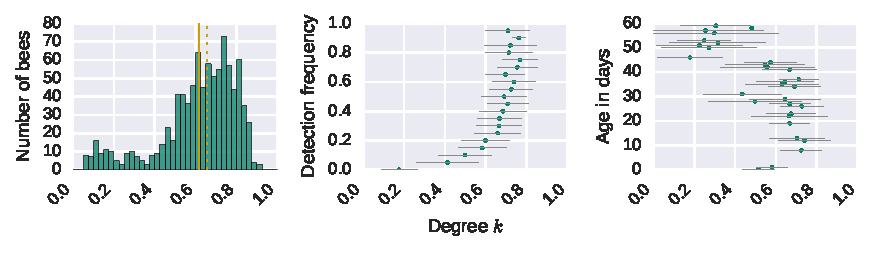
\includegraphics[width=1.0\textwidth]{Figures/n3-stat-degreeAgeDetF.pdf}
	%\caption[Degree]{\textbf{Degree}}
	%\label{fig:n3-degree}
	\end{subfigure}
	\begin{subfigure}[b]{1.0\textwidth}
	\centering
	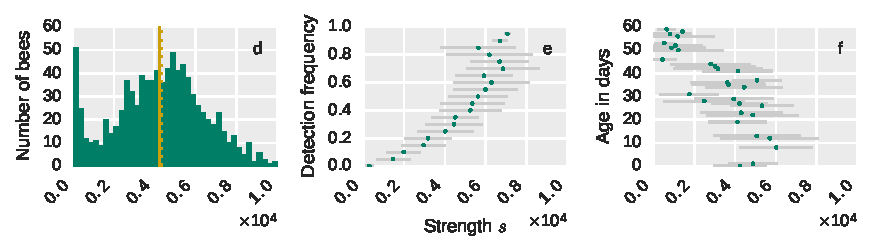
\includegraphics[width=1.0\textwidth]{Figures/n3-stat-strengthAgeDetF.pdf}
	%\caption[Strength]{\textbf{Strength}}
	%\label{fig:n3-strength}
	\end{subfigure}
	\begin{subfigure}[b]{1.0\textwidth}
	\centering
	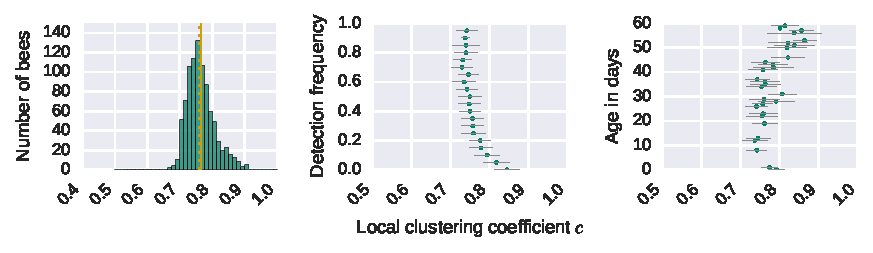
\includegraphics[width=1.0\textwidth]{Figures/n3-stat-lccAgeDetF.pdf}
	%\caption[Local clustering coefficient]{\textbf{Local clustering coefficient}}
	%\label{fig:n3-lcc}
	\end{subfigure}
	\begin{subfigure}[b]{1.0\textwidth}
	\centering
	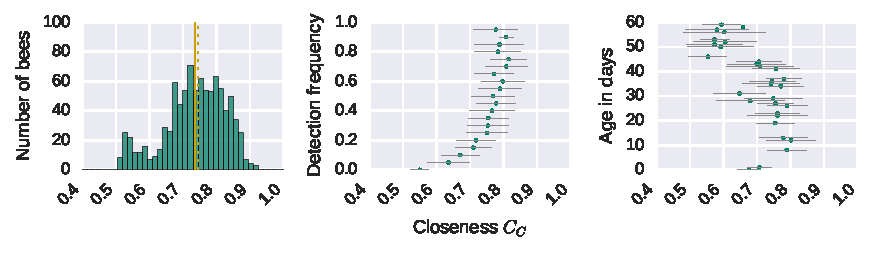
\includegraphics[width=1.0\textwidth]{Figures/n3-stat-closenessAgeDetF.pdf}
	%\caption[Closeness Centrality]{\textbf{Closeness Centrality}}
	%\label{fig:n3-closeness}
	\end{subfigure}
	\begin{subfigure}[b]{1.0\textwidth}
	\centering
	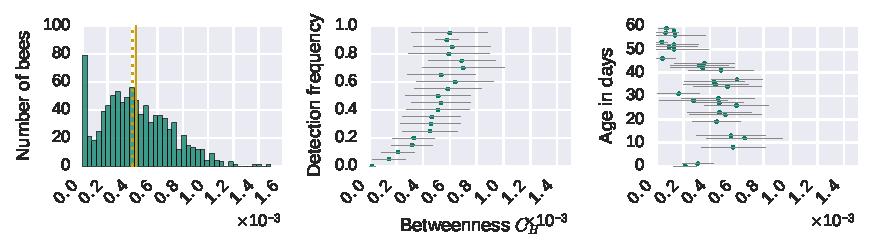
\includegraphics[width=1.0\textwidth]{Figures/n3-stat-betweenAgeDetF.pdf}
	%\caption[Betweeness Centrality]{\textbf{Betweeness Centrality}}
	%\label{fig:n3-between}
	\end{subfigure}
	\caption[Local measures of snapshot~3]{\textbf{Local measures of snapshot~3}}
	\label{fig:n3-degreeStrLCC}
\end{figure}